%%%%%%%%%%%%%%%%%%%%%%%%%%%%%%%%%%%%%%%%%%%%%%%%%%%%%%%%%%%%%%%%%%%%%%%%%%%%%%%%%
\section{Backup Slides}
%%%%%%%%%%%%%%%%%%%%%%%%%%%%%%%%%%%%%%%%%%%%%%%%%%%%%%%%%%%%%%%%%%%%%%%%%%%%%%%%%
\begin{frame}
\frametitle{Strong-Stability-Preserving Runge-Kutta Methods}

\begin{itemize}
  \item A general $s$-stage SSPRK method for discretizing a system
    $\massmatrix\ddt{\solutionvector} = \ssres(\solutionvector,t)$
    is the following:
    \begin{equation}
      \solutionvector^{n+1} = \RKstagesolution^{s} \eqc
    \end{equation}
    \begin{equation}
      \RKstagesolution^i = \left\{\begin{array}{l l}
        \solutionvector^n & i = 0\\
        \RKoldsolutioncoef_i\RKstagesolution^0
        + \RKstagesolutioncoef_i\RKintermediatesolution^i & i\ne 0
      \end{array}\right. \eqc 
    \end{equation}
    \begin{equation}
      \massmatrix\RKintermediatesolution^i = \massmatrix\RKstagesolution^{i-1}
        + \timestepsize\,\ssres(\RKstagetime_i,\RKstagesolution^{i-1})
      \eqc
    \end{equation}
    where $\RKstagetime_i = \timevalue^\timeindex+\RKtimecoef_i\timestepsize$,
  \item An example is the Shu-Osher method (3-stage, 3rd-order-accurate):
    \begin{equation}
      \RKoldsolutioncoef = \left[\begin{array}{c}
        0\\\frac{3}{4}\\\frac{1}{3}\end{array}\right]
        \qquad\RKstagesolutioncoef = \left[\begin{array}{c}
        1\\\frac{1}{4}\\\frac{2}{3}\end{array}\right]
        \qquad c = \left[\begin{array}{c}0\\1\\\frac{1}{2}\end{array}\right] \eqp
    \end{equation}
\end{itemize}

\end{frame}
%%%%%%%%%%%%%%%%%%%%%%%%%%%%%%%%%%%%%%%%%%%%%%%%%%%%%%%%%%%%%%%%%%%%%%%%%%%%%%%%%
\begin{frame}
\frametitle{Low-Order Steady-State Matrix Row Sum}

\begin{itemize}
  \item Recall that $\ssmatrixletter\ij^{L,n}\equiv\ssmatrixletter\ij^{n}
    +\diffusionmatrixletter\ij^{L,n}$. Thus,
      $\sumj\ssmatrixletter\ij^{L,n} = \sumj\ssmatrixletter\ij^{n}
      +\sumj\diffusionmatrixletter\ij^{L,n} \eqp$
  \item Recall the zero-row-sum property of $\diffusionmatrix^{L,n}$:
    \begin{equation}
      \diffusionmatrixletter_{i,i}^{L,n} =
        -\sum_{j\ne i}\diffusionmatrixletter_{i,j}^{L,n}
      \eqc \quad \Rightarrow \quad
        \sumj\diffusionmatrixletter_{i,j}^{L,n} = 0 \eqp
    \end{equation}
  \item Thus $\sumj\ssmatrixletter^{L,n}\ij =
   \sumj \ssmatrixletter^{\timeindex}\ij$:
\begin{equation}
  \sumj\ssmatrixletter^{L,n}\ij = \sumj \intSi
    \left(\mathbf{\consfluxletter}'(\approximatescalarsolution^\timeindex)
      \cdot\nabla\testfunction_j(\x) +
      \reactioncoef(\x)\testfunction_j(\x)\right)\testfunction_i(\x) d\volume \eqp
\end{equation}
  \item Now, using the fact that $\sumj\testfunction_j(\x)=1$
    (and $\nabla 1 = 0$) gives
    \begin{equation}
      \sumj\ssmatrixletter^{L,n}\ij =
        \intSi\reactioncoef(\x)\testfunction_i(\x) d\volume \eqp
    \end{equation}
\end{itemize}

\end{frame}
%%%%%%%%%%%%%%%%%%%%%%%%%%%%%%%%%%%%%%%%%%%%%%%%%%%%%%%%%%%%%%%%%%%%%%%%%%%%%%%%%
\begin{frame}
\frametitle{Limiting Coefficients Definition}

\begin{itemize}
   \item The classic Zalesak limiting strategy starts by separating the
      negative and positive fluxes:
      \begin{equation}
         Q^-_i \leq \sum\limits_{j:\correctionfluxij<0} L\ij \correctionfluxij +
            \sum\limits_{j:\correctionfluxij>0} L\ij \correctionfluxij\leq Q^+_i \eqp
      \end{equation}
   \item Zalesak's limiting coefficients assume that
      all positive fluxes into a node $i$ have the same limiting coefficient
      $L^+_i$ and similarly, negative fluxes have the same limiting coefficient
      $L^-_i$:
      \begin{equation}
        Q^-_i \leq L^-_i \correctionfluxletter^-_i
          + L^+_i \correctionfluxletter^+_i \leq Q^+_i \eqp
      \end{equation}
      where
      \begin{equation}
        \correctionfluxletter_i^- \equiv \sum\limits_{j:\correctionfluxij<0}
          \correctionfluxij \eqc \qquad
        \correctionfluxletter_i^+ \equiv \sum\limits_{j:\correctionfluxij>0}
          \correctionfluxij \eqp
      \end{equation}
   \item As a conservative bound for $L^+_i$, contributions from negative fluxes
      are ignored (pretending $L_i^-=0$), giving
      $L^+_i \leq \frac{Q_i^+}{\correctionfluxletter_i^+}$
      and similarly for $L^-_i$ and the lower bound.
\end{itemize}

\end{frame}
%%%%%%%%%%%%%%%%%%%%%%%%%%%%%%%%%%%%%%%%%%%%%%%%%%%%%%%%%%%%%%%%%%%%%%%%%%%%%%%%%
\begin{frame}
\frametitle{Limiting Coefficients Definition (Cont.)}

\begin{itemize}
   \item Then, recalling that limiting coefficients are not greater than unity:
      \begin{equation}
         L_i^\pm \equiv\left\{
            \begin{array}{l l}
               1 & \correctionfluxletter_i^\pm = 0\\
               \min\left(1,\frac{Q_i^\pm}{\correctionfluxletter_i^\pm}\right) &
                 \correctionfluxletter_i^\pm \ne 0
            \end{array}
            \right. \eqp
      \end{equation}
   \item However, to limit fluxes conservatively, limited correction fluxes must
      be equal and opposite:
      \begin{equation}
        L\ij \correctionfluxij = -L_{j,i}
          \MakeUppercase{\correctionfluxletter}_{j,i} \eqp
      \end{equation}
      Since $\correctionfluxij$ happens to be skew symmetric
      ($\MakeUppercase{\correctionfluxletter}_{j,i}=-\correctionfluxij$) due to the
      chosen flux decomposition, the limiting coefficients must be symmetric:
      $L_{j,i} = L\ij$.
\end{itemize}

\end{frame}
%%%%%%%%%%%%%%%%%%%%%%%%%%%%%%%%%%%%%%%%%%%%%%%%%%%%%%%%%%%%%%%%%%%%%%%%%%%%%%%%%
\begin{frame}
\frametitle{Limiting Coefficients Definition (Cont.)}

\begin{itemize}
   \item Thus when deciding the limiting coefficient $L\ij$ for a flux $\correctionfluxij$, 
      one must not only consider the bounds for $i$ but also the bounds for $j$.
      Specifically, a positive flux $\correctionfluxij$ risks violating $Q_i^+$ and $Q_j^-$.
      Putting everything together,
      \begin{equation}
         L\ij \equiv\left\{
            \begin{array}{l l}
               \min(L_i^+,L_j^-) & \correctionfluxij \geq 0\\
               \min(L_i^-,L_j^+) & \correctionfluxij < 0
            \end{array}
            \right. \eqp
      \end{equation}
\end{itemize}

\end{frame}
%%%%%%%%%%%%%%%%%%%%%%%%%%%%%%%%%%%%%%%%%%%%%%%%%%%%%%%%%%%%%%%%%%%%%%%%%%%%%%%%%%
%\begin{frame}
%\frametitle{Comparison of Time Discretizations}
%\framesubtitle{CFL = 0.8, 32 cells}
%
%\begin{center}
%   \includegraphics[width=0.8\textwidth]
%     {\contentdir/results/transport/time_methods/compare_time_methods.pdf}
%\end{center}
%
%\end{frame}
%%%%%%%%%%%%%%%%%%%%%%%%%%%%%%%%%%%%%%%%%%%%%%%%%%%%%%%%%%%%%%%%%%%%%%%%%%%%%%%%%%
%\begin{frame}
%\frametitle{Backward Euler Galerkin FCT for Different CFL Numbers}
%
%\begin{center}
%   \includegraphics[width=0.9\textwidth]
%     {\contentdir/results/transport/compare_cfl/compare_cfl.pdf}
%\end{center}
%
%\end{frame}
%%%%%%%%%%%%%%%%%%%%%%%%%%%%%%%%%%%%%%%%%%%%%%%%%%%%%%%%%%%%%%%%%%%%%%%%%%%%%%%%%
\begin{frame}
\frametitle{2-D Void-to-Absorber Test Problem}
\framesubtitle{Number of Cells vs. Iterations Study, Steady-State}

\begin{center}
\begin{table}[h]
\caption{EV and FCT Iterations Required for EV-FCT Solution}
\begin{tabular}{c c c}\toprule
$N_{cell}$ & \emph{EV} & \emph{FCT}\\\midrule
 64 & 97 & 716\\
256 & -- & \textcolor{red}{\textbf{FAIL}}\\
\bottomrule\end{tabular}
\end{table}
\end{center}

\end{frame}
%%%%%%%%%%%%%%%%%%%%%%%%%%%%%%%%%%%%%%%%%%%%%%%%%%%%%%%%%%%%%%%%%%%%%%%%%%%%%%%%%
\begin{frame}
\frametitle{3-D Void-to-Absorber Test Problem}
\framesubtitle{Normally-Incident Wave from Void to Absorber Octant, FE}

\begin{figure}[h]
   \centering
   \begin{subfigure}{0.45\textwidth}
      \centering
      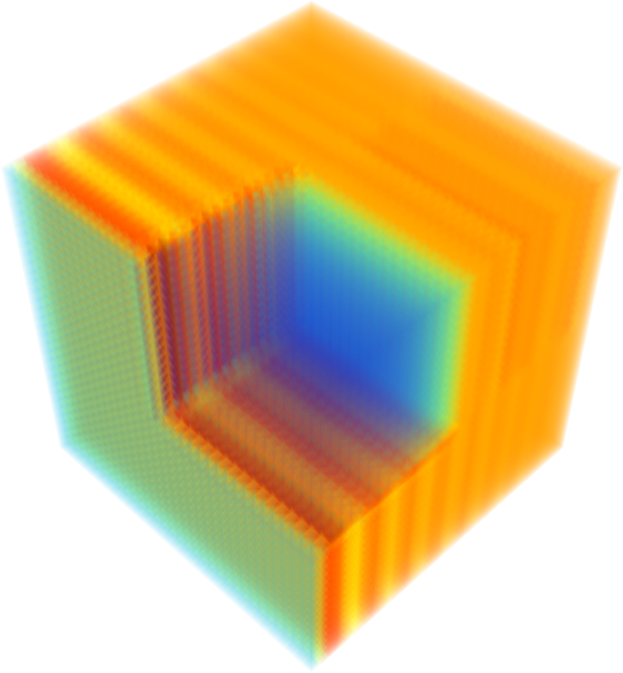
\includegraphics[width=\textwidth]{./figures/Gal_3D.png}
      \caption{Galerkin}
   \end{subfigure}
   \begin{subfigure}{0.45\textwidth}
      \centering
      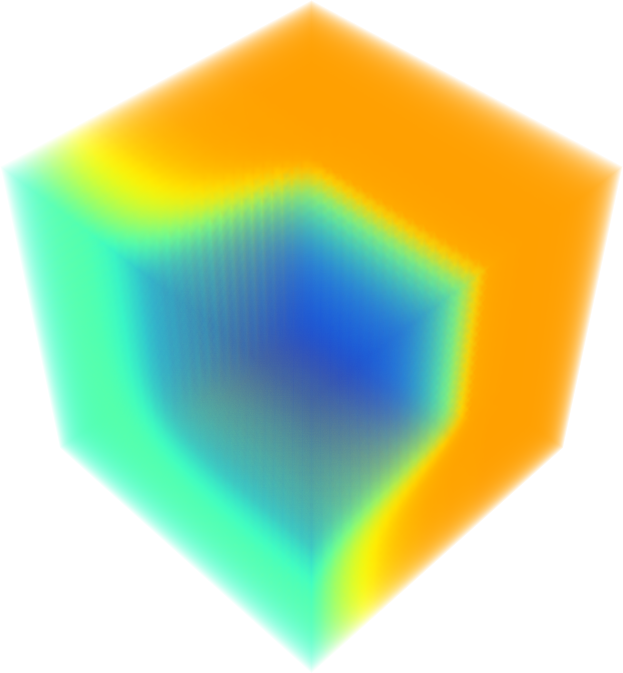
\includegraphics[width=\textwidth]{./figures/GalFCT_3D.png}
      \caption{Galerkin-FCT}
   \end{subfigure}
\end{figure}

\end{frame}
%%%%%%%%%%%%%%%%%%%%%%%%%%%%%%%%%%%%%%%%%%%%%%%%%%%%%%%%%%%%%%%%%%%%%%%%%%%%%%%%%
\begin{frame}
\frametitle{Skew-Incident Void-to-Absorber Test Problem}
\framesubtitle{Skew-Incident Wave from Void to Absorber Quadrant}

\begin{figure}[h]
   \centering
   \begin{subfigure}{0.3\textwidth}
      \centering
      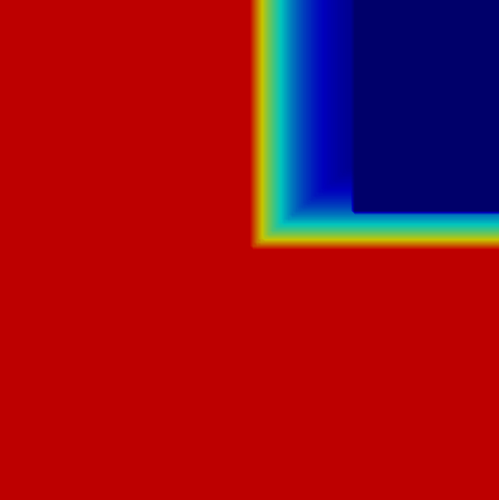
\includegraphics[width=0.8\textwidth]{./figures/skew_exact.png}
      \caption{Exact}
   \end{subfigure}
   \begin{subfigure}{0.3\textwidth}
      \centering
      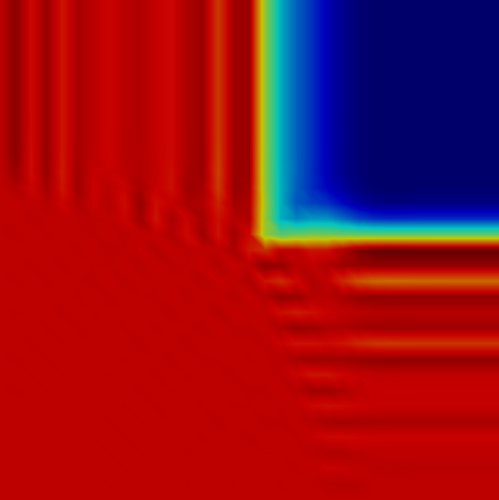
\includegraphics[width=0.8\textwidth]{./figures/skew_Gal.png}
      \caption{Galerkin}
   \end{subfigure}
   \begin{subfigure}{0.3\textwidth}
      \centering
      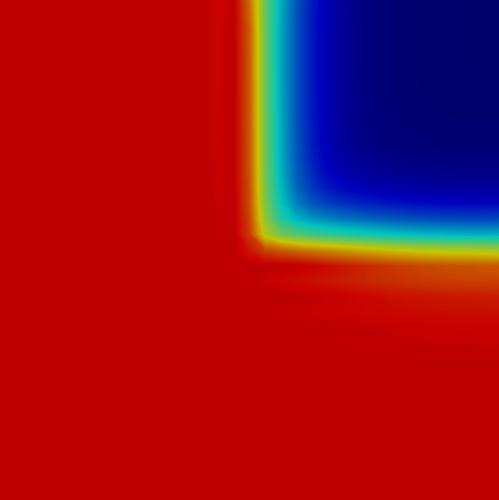
\includegraphics[width=0.8\textwidth]{./figures/skew_GalFCT.png}
      \caption{Galerkin-FCT}
   \end{subfigure}
   \begin{subfigure}{0.3\textwidth}
      \centering
      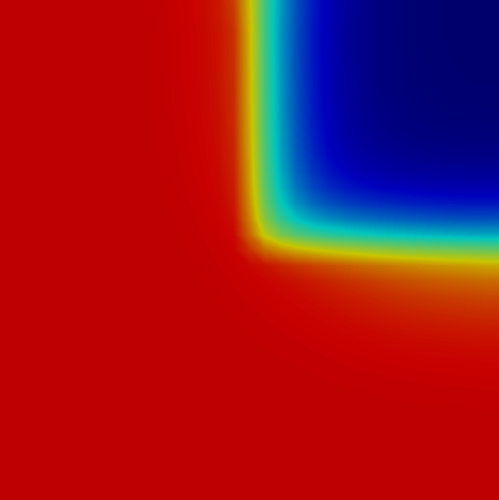
\includegraphics[width=0.8\textwidth]{./figures/skew_low.png}
      \caption{Low-order}
   \end{subfigure}
   \begin{subfigure}{0.3\textwidth}
      \centering
      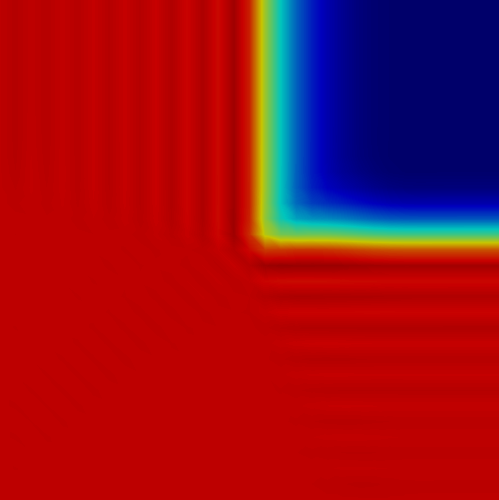
\includegraphics[width=0.8\textwidth]{./figures/skew_EV.png}
      \caption{EV}
   \end{subfigure}
   \begin{subfigure}{0.3\textwidth}
      \centering
      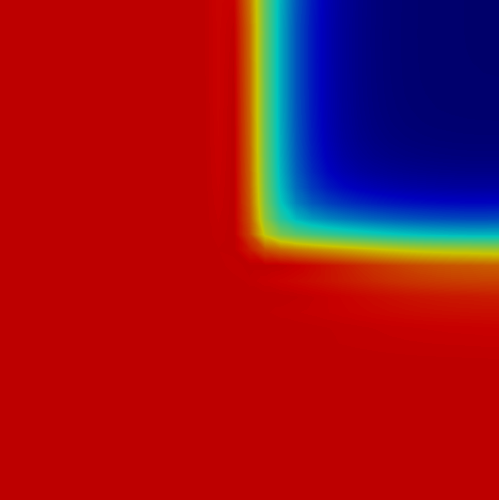
\includegraphics[width=0.8\textwidth]{./figures/skew_EVFCT.png}
      \caption{EV-FCT}
   \end{subfigure}
\end{figure}

\end{frame}
%%%%%%%%%%%%%%%%%%%%%%%%%%%%%%%%%%%%%%%%%%%%%%%%%%%%%%%%%%%%%%%%%%%%%%%%%%%%%%%%%
\begin{frame}
\frametitle{Glance-in-Void Test Problem}
\framesubtitle{Number of Cells vs. Iterations Study, Steady-State}

\begin{center}
\begin{table}[h]
\caption{EV and FCT Iterations Required for EV-FCT Solution}
\begin{tabular}{c c c}\toprule
$N_{cell}$ & \emph{EV} & \emph{FCT}\\\midrule
  64 &   32 & 9284\\
 256 &   59 &  440\\
1024 & 1072 & 3148\\
4096 &   -- & \textcolor{red}{\textbf{FAIL}}\\
\bottomrule\end{tabular}
\end{table}
\end{center}

\end{frame}
%%%%%%%%%%%%%%%%%%%%%%%%%%%%%%%%%%%%%%%%%%%%%%%%%%%%%%%%%%%%%%%%%%%%%%%%%%%%%%%%%
\begin{frame}
\frametitle{Source-Void-to-Absorber Test Problem}
\framesubtitle{Left Half: Source in Vacuum, Right Half: No Source in Absorber}

\begin{center}
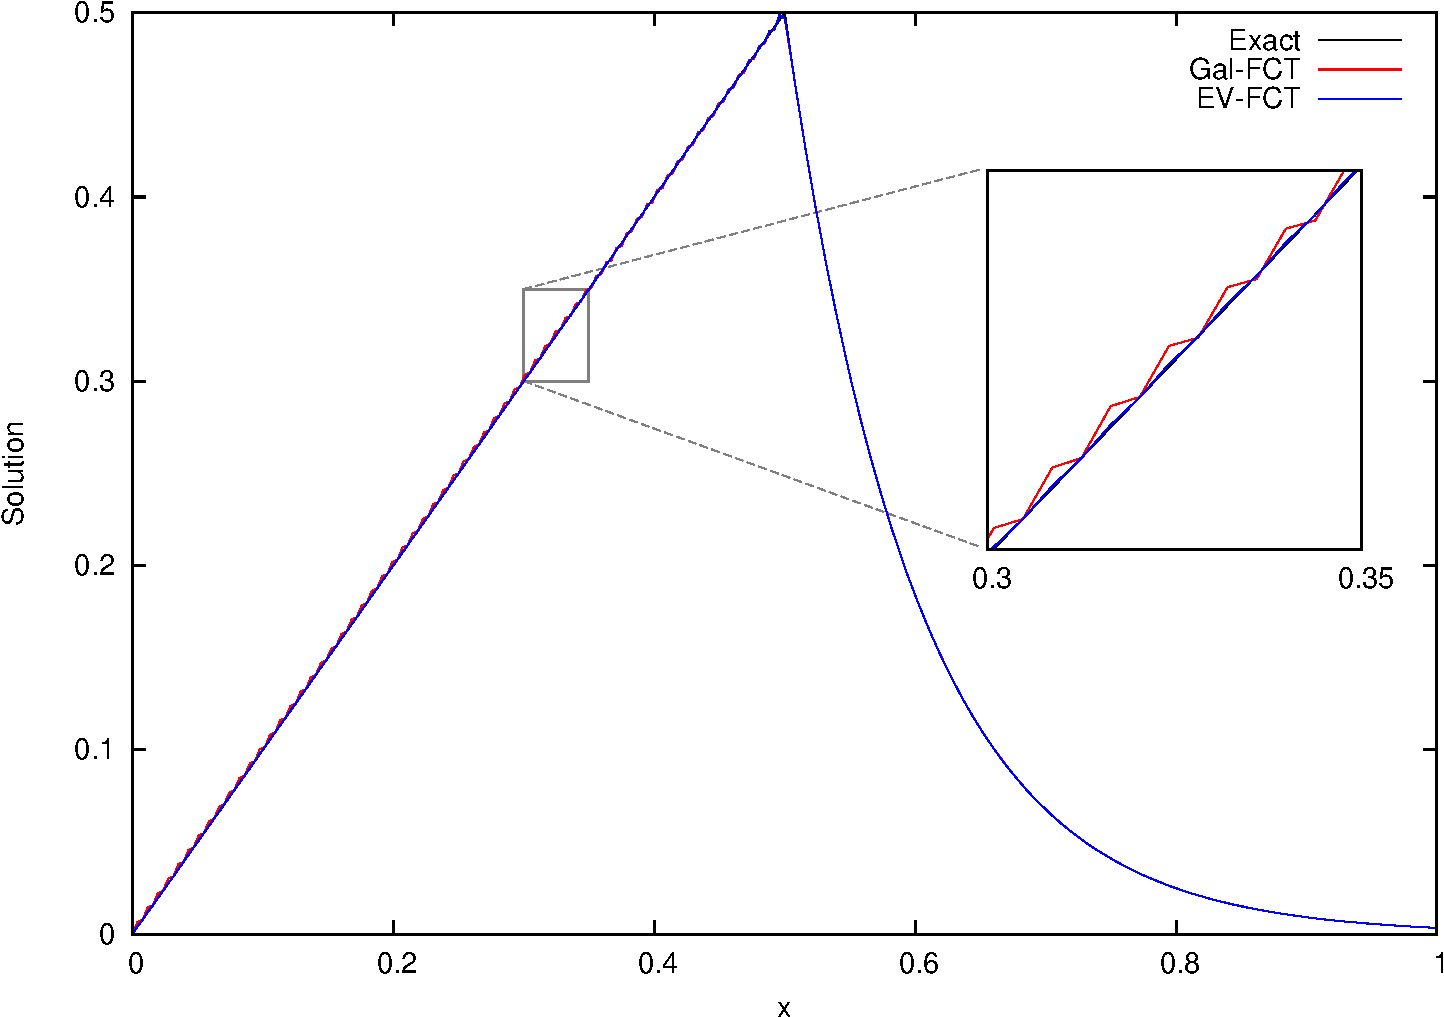
\includegraphics[height=0.8\textheight]{./figures/sourcevoid_FCT_comparison.pdf}
\end{center}

\end{frame}
%%%%%%%%%%%%%%%%%%%%%%%%%%%%%%%%%%%%%%%%%%%%%%%%%%%%%%%%%%%%%%%%%%%%%%%%%%%%%%%%%
\begin{frame}
\frametitle{1-D Dam Break Test Problem}
\framesubtitle{Phase Diagram, FE, 32 cells}

\begin{center}
   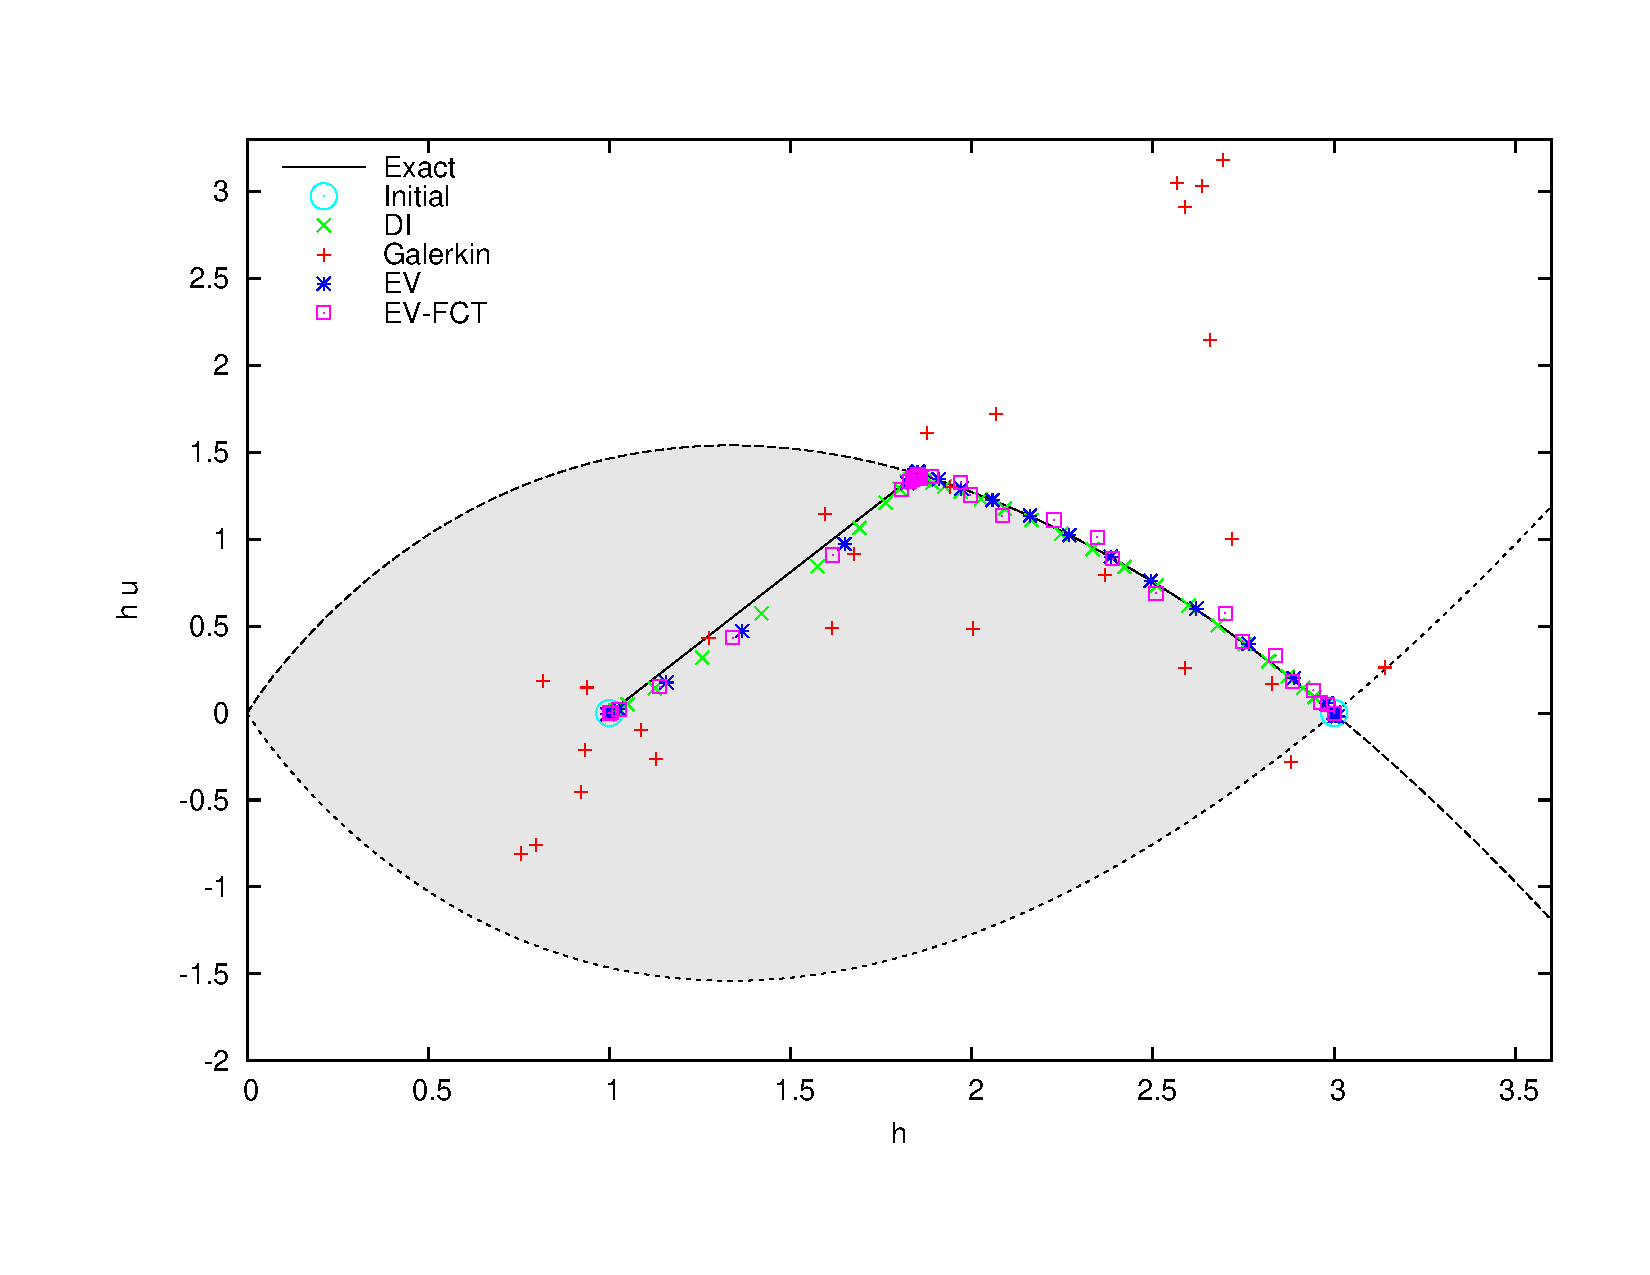
\includegraphics[width=0.9\textwidth]
     {figures/phase_all_FE_32cells.pdf}
\end{center}

\end{frame}
